\documentclass[12pt]{article}
\usepackage{amsmath, amssymb}
\usepackage{xcolor}
\usepackage{tikz}

\begin{document}

\begin{center}
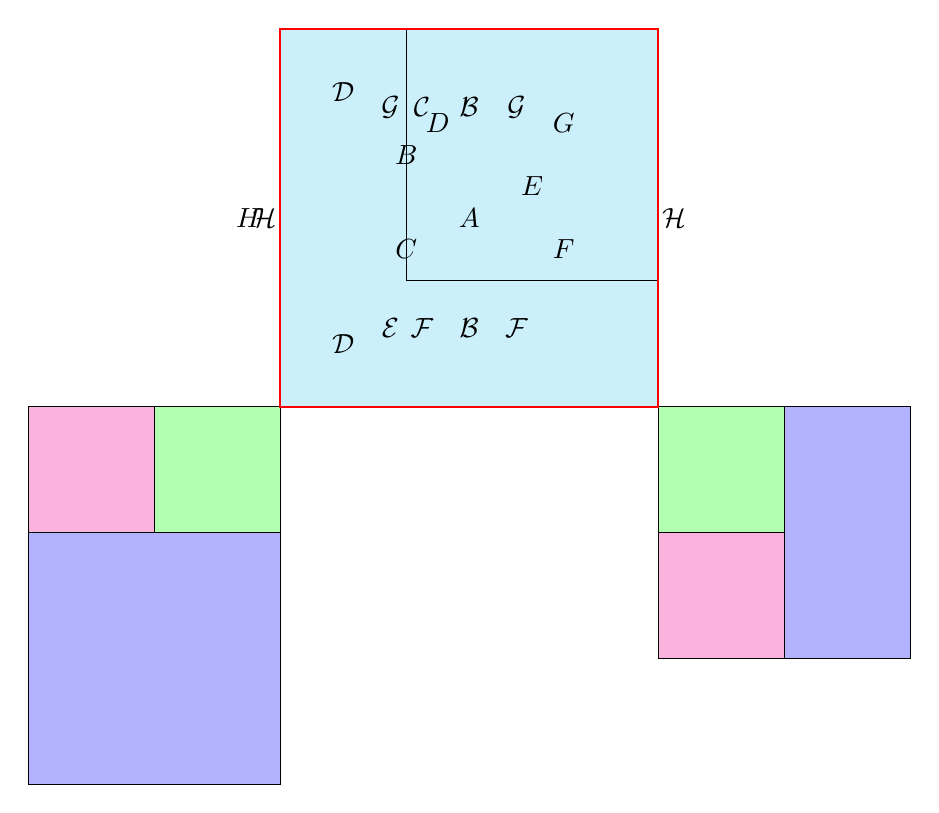
\begin{tikzpicture}[scale=0.8]
    % Define the coordinates for each of the 8 regions
    \coordinate (A) at (-3, -3);
    \coordinate (B) at (3, -3);
    \coordinate (C) at (-3, 3);
    \coordinate (D) at (3, 3);
    
    % Draw the boundaries of each region
    \draw[fill=cyan!20] (A) rectangle ++(6, 6); % Region A
    \draw[fill=blue!30] (A) rectangle ++(-4, -6); % Region B
    \draw[fill=magenta!30] (A) rectangle ++(-4, -2); % Region C
    \draw[fill=green!30] (A) rectangle ++(-2, -2); % Region D
    \draw[fill=blue!30] (B) rectangle ++(4, -4); % Region E
    \draw[fill=magenta!30] (B) rectangle ++(2, -4); % Region F
    \draw[fill=green!30] (B) rectangle ++(2, -2); % Region G
    \draw[fill=cyan!20] (D) rectangle ++(-4, -4); % Region H
    
    % Label the regions
    \node at (0, 0) {$A$};
    \node at (-1, 1) {$B$};
    \node at (-1, -0.5) {$C$};
    \node at (-0.5, 1.5) {$D$};
    \node at (1, 0.5) {$E$};
    \node at (1.5, -0.5) {$F$};
    \node at (1.5, 1.5) {$G$};
    \node at (-3.5, 0) {$H$};
    
    % Draw the red boundary line
    \draw[red, thick] (A) rectangle ++(6, 6);
    
    % Add the set labels
    \node at (0, 1.75) {$\mathcal{B}$};
    \node at (0, -1.75) {$\mathcal{B}$};
    \node at (-0.75, 1.75) {$\mathcal{C}$};
    \node at (-1.25, 1.75) {$\mathcal{G}$};
    \node at (0.75, 1.75) {$\mathcal{G}$};
    \node at (-0.75, -1.75) {$\mathcal{F}$};
    \node at (-1.25, -1.75) {$\mathcal{E}$};
    \node at (0.75, -1.75) {$\mathcal{F}$};
    \node at (-3.25, 0) {$\mathcal{H}$};
    \node at (3.25, 0) {$\mathcal{H}$};
    \node at (-2, 2) {$\mathcal{D}$};
    \node at (-2, -2) {$\mathcal{D}$};
\end{tikzpicture}
\end{center}

\end{document}